\documentclass[11pt,a4paper]{report}
\usepackage[textwidth=37em,vmargin=30mm]{geometry}
\usepackage{calc,xunicode,amsmath,amssymb,paralist,enumitem,tabu,booktabs,datetime2,xeCJK,xeCJKfntef,listings}
\usepackage{tocloft,fancyhdr,tcolorbox,xcolor,graphicx,eso-pic,xltxtra,xelatexemoji}

\newcommand{\envyear}[0]{2025}
\newcommand{\envdatestr}[0]{2025-06-07}
\newcommand{\envfinaldir}[0]{webdb/2025/20250607/final}

\usepackage[hidelinks]{hyperref}
\hypersetup{
    colorlinks=false,
    pdfpagemode=FullScreen,
    pdftitle={Web Digest - \envdatestr}
}

\setlength{\cftbeforechapskip}{10pt}
\renewcommand{\cftchapfont}{\rmfamily\bfseries\large\raggedright}
\setlength{\cftbeforesecskip}{2pt}
\renewcommand{\cftsecfont}{\sffamily\small\raggedright}

\setdefaultleftmargin{2em}{2em}{1em}{1em}{1em}{1em}

\usepackage{xeCJK,xeCJKfntef}
\xeCJKsetup{PunctStyle=plain,RubberPunctSkip=false,CJKglue=\strut\hskip 0pt plus 0.1em minus 0.05em,CJKecglue=\strut\hskip 0.22em plus 0.2em}
\XeTeXlinebreaklocale "zh"
\XeTeXlinebreakskip = 0pt


\setmainfont{Brygada 1918}
\setromanfont{Brygada 1918}
\setsansfont{IBM Plex Sans}
\setmonofont{JetBrains Mono NL}
\setCJKmainfont{Noto Serif CJK SC}
\setCJKromanfont{Noto Serif CJK SC}
\setCJKsansfont{Noto Sans CJK SC}
\setCJKmonofont{Noto Sans CJK SC}

\setlength{\parindent}{0pt}
\setlength{\parskip}{8pt}
\linespread{1.15}

\lstset{
	basicstyle=\ttfamily\footnotesize,
	numbersep=5pt,
	backgroundcolor=\color{black!5},
	showspaces=false,
	showstringspaces=false,
	showtabs=false,
	tabsize=2,
	captionpos=b,
	breaklines=true,
	breakatwhitespace=true,
	breakautoindent=true,
	linewidth=\textwidth
}






\newcommand{\coverpic}[2]{
    % argv: itemurl, authorname
    Cover photo by #2~~(\href{#1}{#1})
}
\newcommand{\makeheader}[0]{
    \begin{titlepage}
        % \newgeometry{hmargin=15mm,tmargin=21mm,bmargin=12mm}
        \begin{center}
            
            \rmfamily\scshape
            \fontspec{BaskervilleF}
            \fontspec{Old Standard}
            \fontsize{59pt}{70pt}\selectfont
            WEB\hfill DIGEST
            
            \vfill
            % \vskip 30pt
            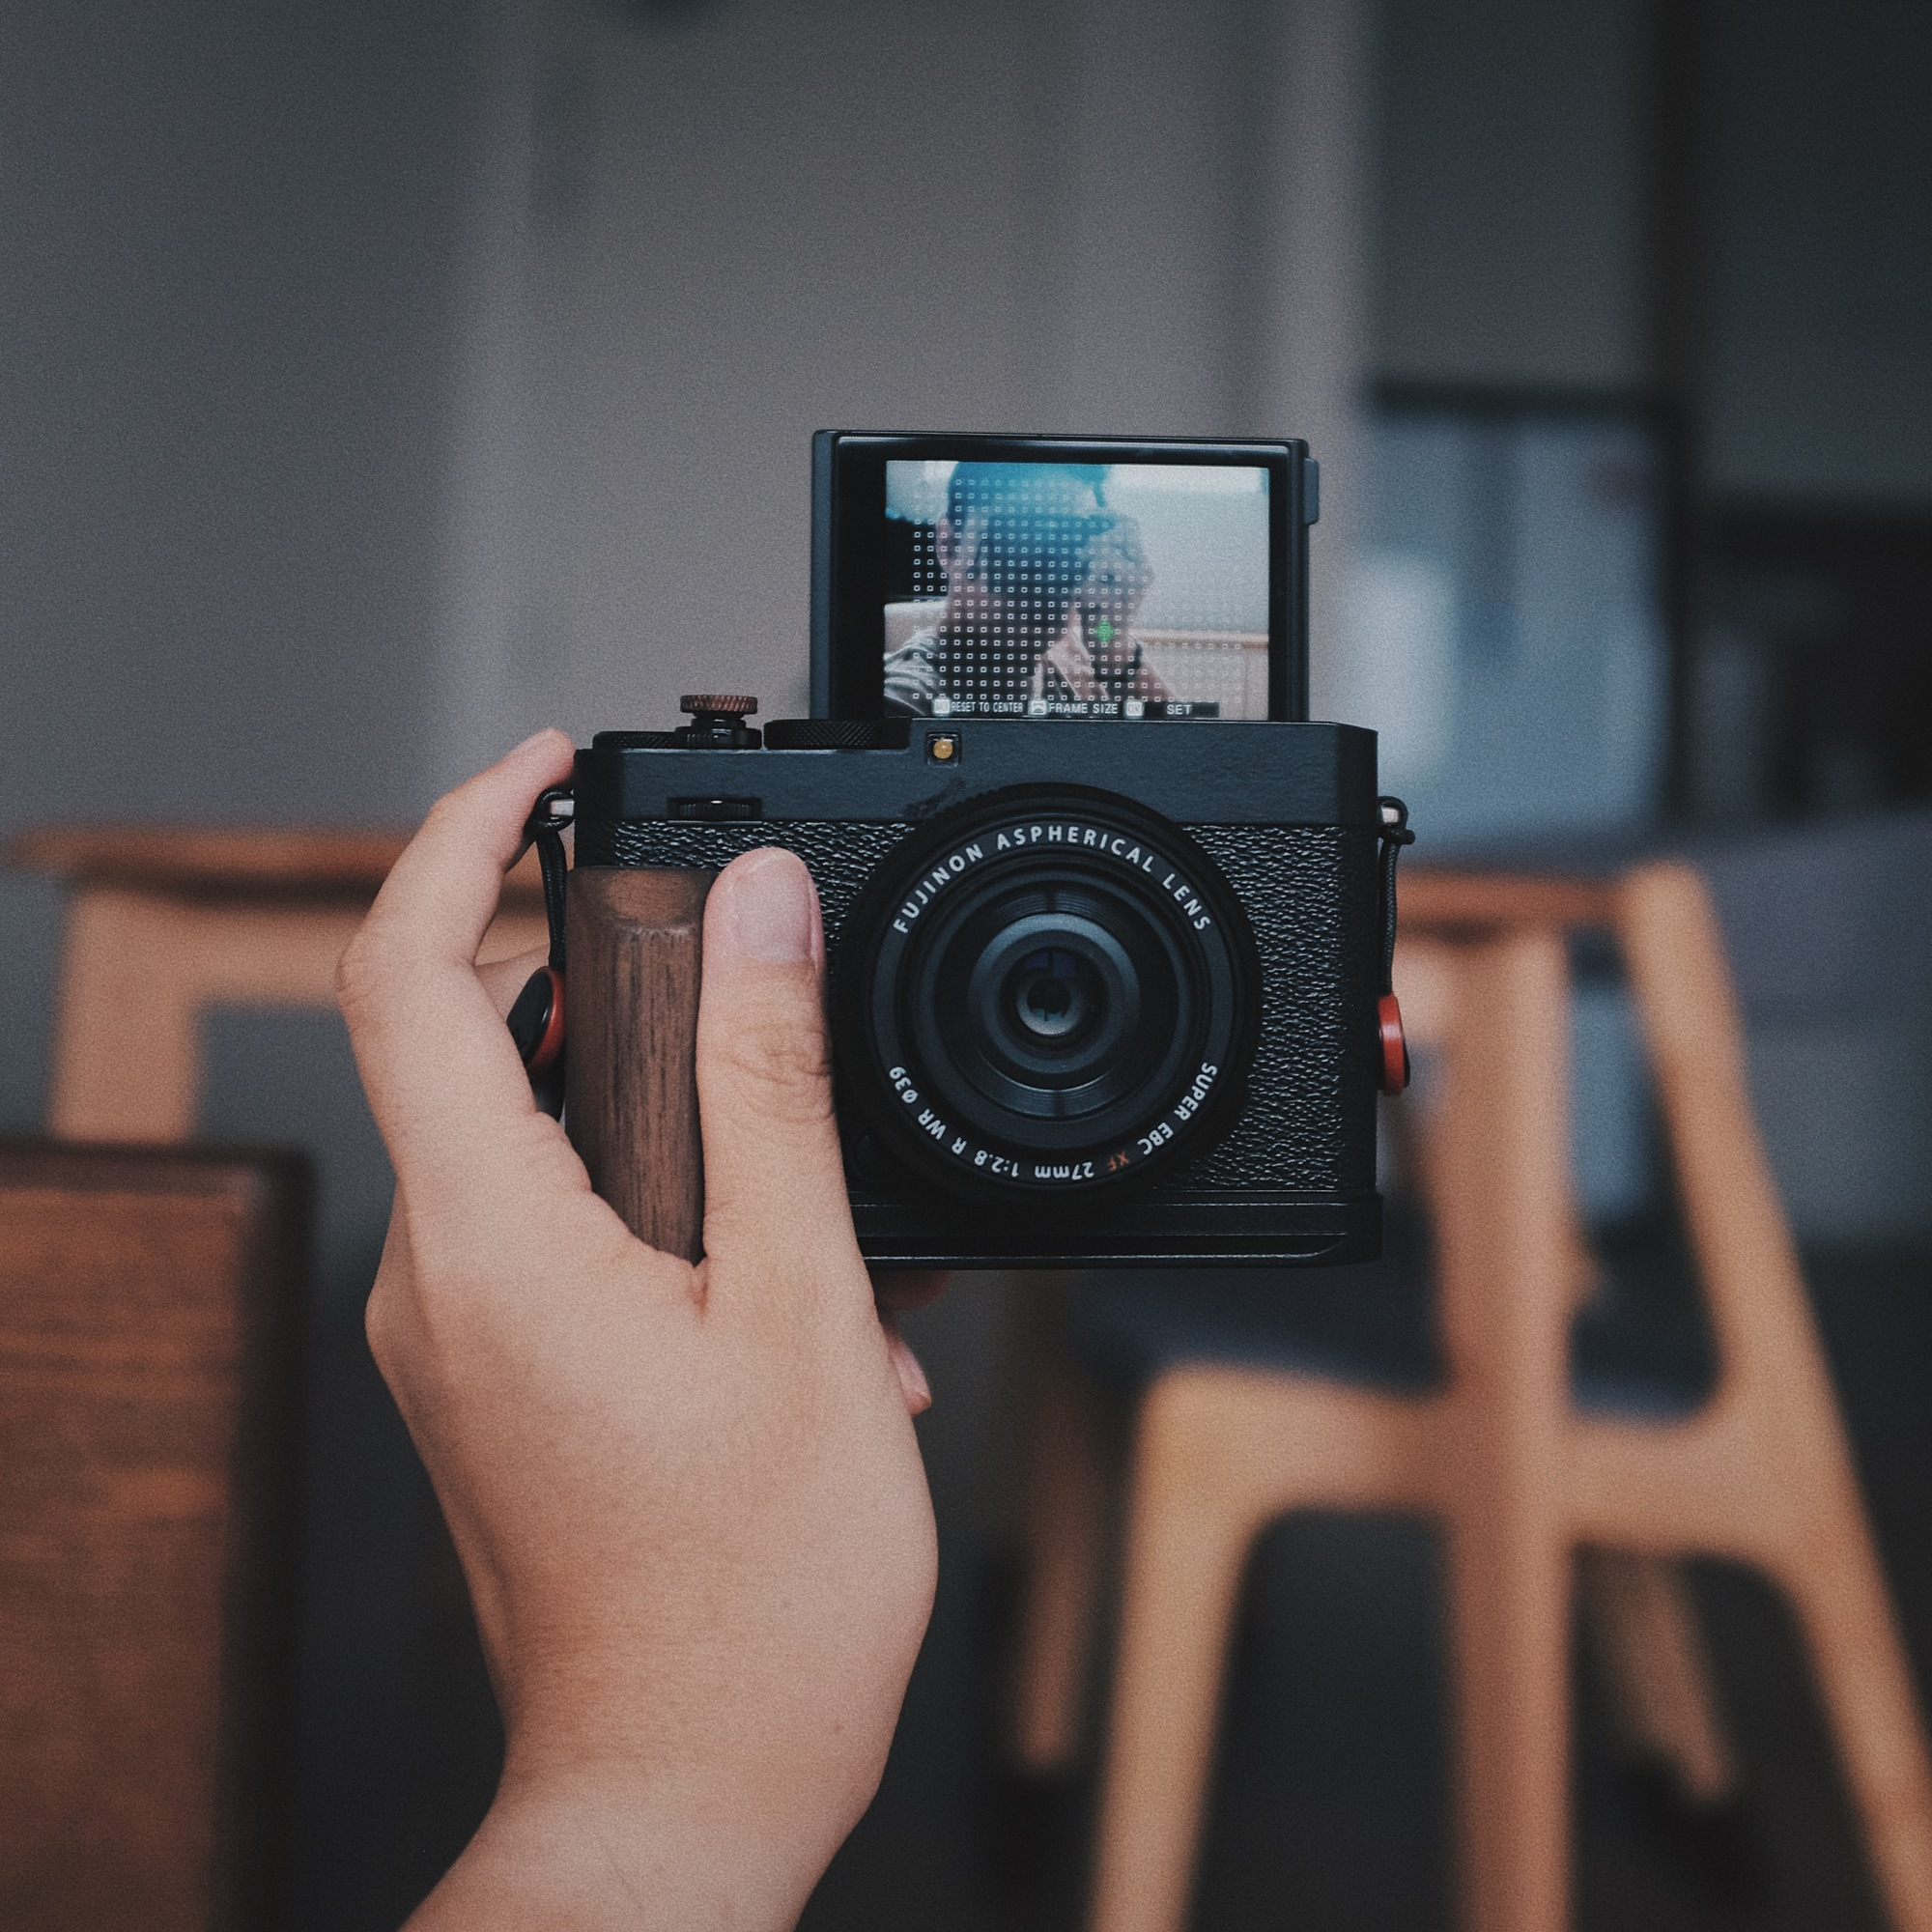
\includegraphics[width=\linewidth]{\envfinaldir/coverpic-prod.jpg}\par
            % \vskip 30pt
            \vfill

            \normalsize\rmfamily\scshape
            \copyright{} The Web Digest Project \hfill\large \envdatestr
        \end{center}
    \end{titlepage}
    % \restoregeometry
}
\newcommand{\simplehref}[1]{%
    \textcolor{blue!80!green}{\href{#1}{#1}}%
}
\renewcommand{\contentsname}{\center\Huge\sffamily\bfseries Contents\par\vskip 20pt}
\newcounter{ipartcounter}
\setcounter{ipartcounter}{0}
\newcommand{\ipart}[1]{
    % \vskip 20pt
    \clearpage
    \stepcounter{ipartcounter}
    \phantomsection
    \addcontentsline{toc}{chapter}{#1}
    % \begin{center}
    %     \Huge
    %     \sffamily\bfseries
    %     #1
    % \end{center}
    % \vskip 20pt plus 7pt
}
\newcounter{ichaptercounter}
\setcounter{ichaptercounter}{0}
\newcommand{\ichapter}[1]{
    % \vskip 20pt
    \clearpage
    \stepcounter{ichaptercounter}
    \phantomsection
    \addcontentsline{toc}{section}{\numberline{\arabic{ichaptercounter}}#1}
    \begin{center}
        \Huge
        \sffamily\bfseries
        #1
    \end{center}
    \vskip 20pt plus 7pt
}
\newcommand{\entrytitlefont}[1]{\subsection*{\raggedright\Large\sffamily\bfseries#1}}
\newcommand{\entryitemGeneric}[2]{
    % argv: title, url
    \parbox{\linewidth}{
        \entrytitlefont{#1}\par\vskip 5pt
        \footnotesize\ttfamily\mdseries
        \simplehref{#2}
    }\vskip 11pt plus 11pt minus 1pt
}
\newcommand{\entryitemGithub}[3]{
    % argv: title, url, desc
    \parbox{\linewidth}{
        \entrytitlefont{#1}\par\vskip 5pt
        \footnotesize\ttfamily\mdseries
        \simplehref{#2}\par\vskip 5pt
        \small\rmfamily\mdseries#3
    }\vskip 11pt plus 11pt minus 1pt
}
\newcommand{\entryitemAp}[3]{
    % argv: title, url, desc
    \parbox{\linewidth}{
        \entrytitlefont{#1}\par\vskip 5pt
        \footnotesize\ttfamily\mdseries
        \simplehref{#2}\par\vskip 5pt
        \small\rmfamily\mdseries#3
    }\vskip 11pt plus 11pt minus 1pt
}
\newcommand{\entryitemHackernews}[3]{
    % argv: title, hnurl, rawurl
    % \parbox{\linewidth}{
    %     \entrytitlefont{#1}\par\vskip 5pt
    %     \footnotesize\ttfamily\mdseries
    %     \simplehref{#3}\par
    %     \textcolor{black!50}{\href{#2}{#2}}
    % }\vskip 11pt plus 11pt minus 1pt
    \begin{minipage}{\linewidth}
            \entrytitlefont{#1}\par\vskip 5pt
            \footnotesize\ttfamily\mdseries
            \simplehref{#3}\par
            \textcolor{black!50}{\href{#2}{#2}}
    \end{minipage}\par\vskip 11pt plus 11pt minus 1pt
}







\begin{document}

\makeheader

\tableofcontents\clearpage




\ipart{Developers}
\ichapter{Hacker News}
\entryitemTwoLinks{Researchers develop `transparent paper' as alternative to plastics}{https://news.ycombinator.com/item?id=44205282}{https://japannews.yomiuri.co.jp/science-nature/technology/20250605-259501/}

\entryitemTwoLinks{United States Digital Service Origins}{https://news.ycombinator.com/item?id=44204277}{https://usdigitalserviceorigins.org/}

\entryitemTwoLinks{A year of funded FreeBSD development}{https://news.ycombinator.com/item?id=44204224}{https://www.daemonology.net/blog/2025-06-06-A-year-of-funded-FreeBSD.html}

\entryitemTwoLinks{SaaS is just vendor lock-in with better branding}{https://news.ycombinator.com/item?id=44203494}{https://rwsdk.com/blog/saas-is-just-vendor-lock-in-with-better-branding}

\entryitemTwoLinks{Researchers find a way to make the HIV virus visible within white blood cells}{https://news.ycombinator.com/item?id=44202664}{https://www.theguardian.com/global-development/2025/jun/05/breakthrough-in-search-for-hiv-cure-leaves-researchers-overwhelmed}

\entryitemTwoLinks{How we decreased GitLab repo backup times from 48 hours to 41 minutes}{https://news.ycombinator.com/item?id=44201975}{https://about.gitlab.com/blog/2025/06/05/how-we-decreased-gitlab-repo-backup-times-from-48-hours-to-41-minutes/}

\entryitemTwoLinks{4-7-8 Breathing}{https://news.ycombinator.com/item?id=44201901}{https://www.breathbelly.com/exercises/4-7-8-breathing}

\entryitemTwoLinks{Meta: Shut down your invasive AI Discover feed}{https://news.ycombinator.com/item?id=44201872}{https://www.mozillafoundation.org/en/campaigns/meta-shut-down-your-invasive-ai-discover-feed-now/}

\entryitemTwoLinks{VPN providers in France ordered to block pirate sports IPTV}{https://news.ycombinator.com/item?id=44201857}{https://torrentfreak.com/major-vpn-providers-ordered-to-block-pirate-sports-streaming-sites-250516/}

\entryitemTwoLinks{Sandia turns on brain-like storage-free supercomputer}{https://news.ycombinator.com/item?id=44201812}{https://blocksandfiles.com/2025/06/06/sandia-turns-on-brain-like-storage-free-supercomputer/}

\entryitemTwoLinks{OpenAI is retaining all ChatGPT logs "indefinitely." Here's who's affected}{https://news.ycombinator.com/item?id=44201785}{https://arstechnica.com/tech-policy/2025/06/openai-confronts-user-panic-over-court-ordered-retention-of-chatgpt-logs/}

\entryitemTwoLinks{An Interactive Guide to Rate Limiting}{https://news.ycombinator.com/item?id=44201583}{https://blog.sagyamthapa.com.np/interactive-guide-to-rate-limiting}

\entryitemTwoLinks{Top researchers leave Intel to build startup with 'the biggest, baddest CPU'}{https://news.ycombinator.com/item?id=44201072}{https://www.oregonlive.com/silicon-forest/2025/06/top-researchers-leave-intel-to-build-startup-with-the-biggest-baddest-cpu.html}

\entryitemTwoLinks{A masochist's guide to web development}{https://news.ycombinator.com/item?id=44200895}{https://sebastiano.tronto.net/blog/2025-06-06-webdev/}

\entryitemTwoLinks{Odyc.js – A tiny JavaScript library for narrative games}{https://news.ycombinator.com/item?id=44200866}{https://odyc.dev}

\entryitemTwoLinks{Small Programs and Languages}{https://news.ycombinator.com/item?id=44200797}{https://ratfactor.com/cards/pl-small}

\entryitemTwoLinks{Dystopian tales of that time when I sold out to Google}{https://news.ycombinator.com/item?id=44200773}{https://wordsmith.social/elilla/deep-in-mordor-where-the-shadows-lie-dystopian-stories-of-my-time-as-a-googler}

\entryitemTwoLinks{Being fat is a trap}{https://news.ycombinator.com/item?id=44200199}{https://federicopereiro.com/fat-trap/}

\entryitemTwoLinks{Doge Developed Error-Prone AI Tool to "Munch" Veterans Affairs Contracts}{https://news.ycombinator.com/item?id=44199887}{https://www.propublica.org/article/trump-doge-veterans-affairs-ai-contracts-health-care}

\entryitemTwoLinks{What you need to know about EMP weapons}{https://news.ycombinator.com/item?id=44199649}{https://www.aardvark.co.nz/daily/2025/0606.shtml}\ichapter{Dribbble}
\entryitemGeneric{\hskip 0pt{}Aquasan}{https://dribbble.com/shots/26100535-Aquasan}

\entryitemGeneric{\hskip 0pt{}Eagle}{https://dribbble.com/shots/26099428-Eagle}

\entryitemGeneric{\hskip 0pt{}Mnp Technologies - Logo Design}{https://dribbble.com/shots/26092034-Mnp-Technologies-Logo-Design}

\entryitemGeneric{\hskip 0pt{}Singular Logo Concept (Unused)}{https://dribbble.com/shots/26091755-Singular-Logo-Concept-Unused}

\entryitemGeneric{\hskip 0pt{}Cre8tera // Website}{https://dribbble.com/shots/26091009-Cre8tera-Website}

\entryitemGeneric{\hskip 0pt{}Cool Pool Logo Design - Letter C Monogram}{https://dribbble.com/shots/26091401-Cool-Pool-Logo-Design-Letter-C-Monogram}

\entryitemGeneric{\hskip 0pt{}Gorilla + Bar Chart Logo}{https://dribbble.com/shots/26092670-Gorilla-Bar-Chart-Logo}

\entryitemGeneric{\hskip 0pt{}zeero logo design}{https://dribbble.com/shots/26087342-zeero-logo-design}

\entryitemGeneric{\hskip 0pt{}Create email inbox composition}{https://dribbble.com/shots/26083118-Create-email-inbox-composition}

\entryitemGeneric{\hskip 0pt{}Shori Brand}{https://dribbble.com/shots/26088139-Shori-Brand}

\entryitemGeneric{\hskip 0pt{}Roaring Bear}{https://dribbble.com/shots/26087788-Roaring-Bear}

\entryitemGeneric{\hskip 0pt{}Eagle}{https://dribbble.com/shots/26085536-Eagle}

\entryitemGeneric{\hskip 0pt{}Hand-drawn illustration pack}{https://dribbble.com/shots/26084735-Hand-drawn-illustration-pack}

\entryitemGeneric{\hskip 0pt{}Dog Mascot Various Poses}{https://dribbble.com/shots/26087977-Dog-Mascot-Various-Poses}

\entryitemGeneric{\hskip 0pt{}Branding Concept for Europe}{https://dribbble.com/shots/26087652-Branding-Concept-for-Europe}

\entryitemGeneric{\hskip 0pt{}B2B Dashboard \& Web App UI UX Design for Carbon Solutions}{https://dribbble.com/shots/26076624-B2B-Dashboard-Web-App-UI-UX-Design-for-Carbon-Solutions}

\entryitemGeneric{\hskip 0pt{}Patriot Logo Design (Unused for Sale)}{https://dribbble.com/shots/26081047-Patriot-Logo-Design-Unused-for-Sale}

\entryitemGeneric{\hskip 0pt{}Heliopoint}{https://dribbble.com/shots/26081987-Heliopoint}

\entryitemGeneric{\hskip 0pt{}Apple}{https://dribbble.com/shots/26084067-Apple}

\entryitemGeneric{\hskip 0pt{}Illustration}{https://dribbble.com/shots/26083223-Illustration}

\entryitemGeneric{\hskip 0pt{}Europe Logo Animation}{https://dribbble.com/shots/26082596-Europe-Logo-Animation}

\entryitemGeneric{\hskip 0pt{}Arc Logo}{https://dribbble.com/shots/26083648-Arc-Logo}

\entryitemGeneric{\hskip 0pt{}Heyo Turns 2!}{https://dribbble.com/shots/26078572-Heyo-Turns-2}

\entryitemGeneric{\hskip 0pt{}Fox Brand Mascot}{https://dribbble.com/shots/26077954-Fox-Brand-Mascot}


\ipart{Developers~~~~(zh-Hans)}
\ichapter{Solidot}
\entryitemGeneric{\hskip 0pt{}海南政府试点跨境加速服务}{https://www.solidot.org/story?sid=81485}

\entryitemGeneric{\hskip 0pt{}在传出 OpenAI 准备收购 Windsurf 后 Anthropic 切断了该公司对其大模型的访问}{https://www.solidot.org/story?sid=81484}

\entryitemGeneric{\hskip 0pt{}亚马逊测试用人形机器人送包裹}{https://www.solidot.org/story?sid=81483}

\entryitemGeneric{\hskip 0pt{}美洲原住民在千年前就以集约化方式种植玉米}{https://www.solidot.org/story?sid=81482}

\entryitemGeneric{\hskip 0pt{}Adobe 发布 Android 版 Photoshop,目前免费测试}{https://www.solidot.org/story?sid=81481}

\entryitemGeneric{\hskip 0pt{}特斯拉汽车销量在欧洲继续下滑}{https://www.solidot.org/story?sid=81480}

\entryitemGeneric{\hskip 0pt{}Wendelstein 7-X 仿星器创下可控核聚变新纪录}{https://www.solidot.org/story?sid=81479}

\entryitemGeneric{\hskip 0pt{}Google Chrome 撤销对中华电信和 Netlock CA 的信任}{https://www.solidot.org/story?sid=81478}

\entryitemGeneric{\hskip 0pt{}随着 Windows 10 即将终止支持,KDE 项目试图吸引微软用户}{https://www.solidot.org/story?sid=81477}

\entryitemGeneric{\hskip 0pt{}草帽星系可能经历过星系合并}{https://www.solidot.org/story?sid=81476}

\entryitemGeneric{\hskip 0pt{}科学家发现一颗位于宜居带的超级地球}{https://www.solidot.org/story?sid=81475}

\entryitemGeneric{\hskip 0pt{}蓬勃发展的克隆动物生意}{https://www.solidot.org/story?sid=81474}

\entryitemGeneric{\hskip 0pt{}Reddit 起诉 Anthropic 违反合同和不公平竞争}{https://www.solidot.org/story?sid=81473}

\entryitemGeneric{\hskip 0pt{}韦伯发现已知最遥远的星系}{https://www.solidot.org/story?sid=81472}

\entryitemGeneric{\hskip 0pt{}Meta Android 应用停止使用移动端口跟踪技术}{https://www.solidot.org/story?sid=81471}

\entryitemGeneric{\hskip 0pt{}为遵守欧盟法律微软给予欧洲用户对 Windows 更多的控制权}{https://www.solidot.org/story?sid=81470}

\entryitemGeneric{\hskip 0pt{}微软测试给记事本添加 Markdown}{https://www.solidot.org/story?sid=81469}

\entryitemGeneric{\hskip 0pt{}科学家确认 2023 年发生的神秘震动源自格陵兰岛海啸}{https://www.solidot.org/story?sid=81468}

\entryitemGeneric{\hskip 0pt{}特朗普政府的 2026 年预算将为商业火星探索拨款逾 10 亿美元}{https://www.solidot.org/story?sid=81467}

\entryitemGeneric{\hskip 0pt{}日本 2024 年新生儿数首次跌破 70 万}{https://www.solidot.org/story?sid=81466}\ichapter{V2EX}
\entryitemGeneric{\hskip 0pt{}[酷工作] [全职实习/可远程] 招聘前端实习生}{https://www.v2ex.com/t/1136977}

\entryitemGeneric{\hskip 0pt{}[问与答] 还会坚持用知乎和 csdn 吗?}{https://www.v2ex.com/t/1136976}

\entryitemGeneric{\hskip 0pt{}[程序员] 🚴‍🚴‍‍主力工具,windows 与 mac 如何选,大伙帮给点建议}{https://www.v2ex.com/t/1136975}

\entryitemGeneric{\hskip 0pt{}[阅读] 2025 五月读演化论 心理 育儿 小说…… 8 本}{https://www.v2ex.com/t/1136974}

\entryitemGeneric{\hskip 0pt{}[程序员] 关于 vscode ssh 远程 Linux 开发的一些问题?大牛们回复我了}{https://www.v2ex.com/t/1136973}

\entryitemGeneric{\hskip 0pt{}[分享创造] ConvoQueen 一个个人对话记录助手,帮助你追踪生活中与他人的聊天,并通过 AI 提供关系洞察}{https://www.v2ex.com/t/1136972}

\entryitemGeneric{\hskip 0pt{}[宽带症候群] 求好用便宜的 usb 4g modem 推荐}{https://www.v2ex.com/t/1136971}

\entryitemGeneric{\hskip 0pt{}[宽带症候群] ipv6 问题,一时间不知道骂谁}{https://www.v2ex.com/t/1136970}

\entryitemGeneric{\hskip 0pt{}[分享发现] 我爸从百度和应用商店下载``个人所得税''被骗四位数的故事}{https://www.v2ex.com/t/1136968}

\entryitemGeneric{\hskip 0pt{}[问与答] 显示器三选一,纠结}{https://www.v2ex.com/t/1136966}

\entryitemGeneric{\hskip 0pt{}[macOS] 大家用 macos 有什么好用的视频播放器吗?}{https://www.v2ex.com/t/1136965}

\entryitemGeneric{\hskip 0pt{}[分享创造] 根据开源项目,做了一个临时邮箱服务 temp-mail.top}{https://www.v2ex.com/t/1136964}

\entryitemGeneric{\hskip 0pt{}[微信] 苹果手机拨号多了微信拨号怎么移除}{https://www.v2ex.com/t/1136961}

\entryitemGeneric{\hskip 0pt{}[职场话题] 技术路线的尽头是不是就是大头兵}{https://www.v2ex.com/t/1136960}

\entryitemGeneric{\hskip 0pt{}[互联网] 王自如回归,你怎么看}{https://www.v2ex.com/t/1136959}

\entryitemGeneric{\hskip 0pt{}[问与答] 有性价比高的充电头推荐吗}{https://www.v2ex.com/t/1136957}

\entryitemGeneric{\hskip 0pt{}[酷工作] 推荐一场不错的 AI 公司联合线上招聘活动}{https://www.v2ex.com/t/1136956}

\entryitemGeneric{\hskip 0pt{}[问与答] 有偿求助,使用 Java 的 rsocket 上传文件}{https://www.v2ex.com/t/1136955}

\entryitemGeneric{\hskip 0pt{}[酷工作] [广州外企招聘] 招聘 Business Analyst 多名, 居家 + 公司混合办公模式}{https://www.v2ex.com/t/1136954}

\entryitemGeneric{\hskip 0pt{}[酷工作] 渣打银行天津、广州 it 岗内推}{https://www.v2ex.com/t/1136953}

\entryitemGeneric{\hskip 0pt{}[OpenAI] MCP 和 agent 发展这么久, AI 帮忙寻找某个地点附近性价比高的酒店的需求好像还是没有很好的满足}{https://www.v2ex.com/t/1136952}

\entryitemGeneric{\hskip 0pt{}[问与答] 2025 还有没有类似 射雕 1.0 的 MMORPG 游戏啊!}{https://www.v2ex.com/t/1136951}

\entryitemGeneric{\hskip 0pt{}[问与答] 今年开始,感觉各平台外卖送货,普遍提前几分钟打电话。}{https://www.v2ex.com/t/1136949}

\entryitemGeneric{\hskip 0pt{}[问与答] 请问速度跟翻译准确度都不错的大模型推荐}{https://www.v2ex.com/t/1136948}

\entryitemGeneric{\hskip 0pt{}[分享创造] 快速构建自己的网络信息聚合,分析,日报平台,附 AI 洞察日报}{https://www.v2ex.com/t/1136947}

\entryitemGeneric{\hskip 0pt{}[程序员] 现在搞 askmanyai 这种还有前途么}{https://www.v2ex.com/t/1136946}

\entryitemGeneric{\hskip 0pt{}[酷工作] 寻前端开发(兼职、实习)一名,对我们做得事情特别感兴趣也可以合伙}{https://www.v2ex.com/t/1136945}

\entryitemGeneric{\hskip 0pt{}[酷工作] 招聘岗位: Next 全栈开发工程师(C 端 / 广州天河)}{https://www.v2ex.com/t/1136944}

\entryitemGeneric{\hskip 0pt{}[生活] 新生儿监护摄像头方案分享}{https://www.v2ex.com/t/1136943}

\entryitemGeneric{\hskip 0pt{}[分享创造] 分享一个 deepseek 导出 word 和图片的油猴脚本}{https://www.v2ex.com/t/1136942}

\entryitemGeneric{\hskip 0pt{}[问与答] 趁着 AI 蛊王横空出世之前, 有无可能从中挖掘一些商业流量?}{https://www.v2ex.com/t/1136941}

\entryitemGeneric{\hskip 0pt{}[问与答] 便宜办公椅久坐腰酸,求推荐靠谱的靠腰垫}{https://www.v2ex.com/t/1136939}

\entryitemGeneric{\hskip 0pt{}[YouTube] V 友们, Youtube 还有好的广告拦截工具吗}{https://www.v2ex.com/t/1136937}

\entryitemGeneric{\hskip 0pt{}[酷工作] 广州汇丰银行 - TEKsystems - 招聘 Business Analyst}{https://www.v2ex.com/t/1136936}

\entryitemGeneric{\hskip 0pt{}[问与答] 搞钱能力堪忧}{https://www.v2ex.com/t/1136935}

\entryitemGeneric{\hskip 0pt{}[NAS] 求解群晖 docker container 内访问外网问题}{https://www.v2ex.com/t/1136934}

\entryitemGeneric{\hskip 0pt{}[酷工作] [深圳] ClackyAI Coding 急招资深前端开发工程师(AI 方向,高薪+原始股)}{https://www.v2ex.com/t/1136933}

\entryitemGeneric{\hskip 0pt{}[问与答] 谁知道 LoL 手游的橙色原石怎么获得?}{https://www.v2ex.com/t/1136930}

\entryitemGeneric{\hskip 0pt{}[微信] 微信如何悄无声息的屏蔽一个人的?}{https://www.v2ex.com/t/1136929}

\entryitemGeneric{\hskip 0pt{}[酷工作] 西雅图电商 AI 公司 Pipe17 重启招聘(技术支持工程师)!加入高速发展的全球化团队的机会来了!}{https://www.v2ex.com/t/1136928}

\entryitemGeneric{\hskip 0pt{}[奇思妙想] 2021 年底/22 年初我写的一些关于房地产的思考含金量还在上升}{https://www.v2ex.com/t/1136927}

\entryitemGeneric{\hskip 0pt{}[程序员] Augment 貌似被墙!}{https://www.v2ex.com/t/1136925}

\entryitemGeneric{\hskip 0pt{}[硬件] 2025 年了,还有人用 esxi6.7 做虚拟化底层系统吗}{https://www.v2ex.com/t/1136924}

\entryitemGeneric{\hskip 0pt{}[Linux] 感觉 Linux 桌面也没什么用}{https://www.v2ex.com/t/1136923}

\entryitemGeneric{\hskip 0pt{}[酷工作] LongBridge 长桥证券内推,杭州、成都等众多城市等你来投~}{https://www.v2ex.com/t/1136922}

\entryitemGeneric{\hskip 0pt{}[求职] 3 年+ Web3 经验, 10+ 全栈经验}{https://www.v2ex.com/t/1136920}

\entryitemGeneric{\hskip 0pt{}[VPS] tx cloud 国内 轻量}{https://www.v2ex.com/t/1136919}

\entryitemGeneric{\hskip 0pt{}[问与答] DIY 键盘入门,手搓成本最低的方式是?}{https://www.v2ex.com/t/1136918}

\entryitemGeneric{\hskip 0pt{}[问与答] 闲鱼上看到的电脑,可以入吗?}{https://www.v2ex.com/t/1136917}

\entryitemGeneric{\hskip 0pt{}[问与答] 大佬们,加速度数据怎么存好点}{https://www.v2ex.com/t/1136913}


\ipart{Generic News}
\ichapter{AP News}
\entryitemWithDescription{\hskip 0pt{}Michaels completes acquisition of Joann's intellectual property and fan-favorite labels}{https://apnews.com/article/c57cae0101fc31da0661c69691066bf5}{}

\entryitemWithDescription{\hskip 0pt{}Midea recalling 1.7 million of its popular air conditioners due to mold concern}{https://apnews.com/article/59e18fb2ecce43711d794c2ca7802ce8}{}

\entryitemWithDescription{\hskip 0pt{}Police consider whether `King of the Hill' actor's sexual orientation played a role in his killing}{https://apnews.com/article/741890b752b0a2a4f8fa8a661bc0c5a1}{}

\entryitemWithDescription{\hskip 0pt{}What to know about the much-anticipated Nintendo Switch 2 on launch day}{https://apnews.com/article/5c8164c9f4dbac998962de29f24947d2}{}

\entryitemWithDescription{\hskip 0pt{}FanDuel bans bettor over heckling incident with Olympic champion sprinter Gabby Thomas}{https://apnews.com/article/d226103292fdf6c019f0c71435e9745e}{}

\entryitemWithDescription{\hskip 0pt{}Ex-White House press secretary Karine Jean-Pierre left Democratic Party, publisher of her book says}{https://apnews.com/article/fbb44b9eb3bb56f6ab8ef02bd7ffa042}{}

\entryitemWithDescription{\hskip 0pt{}Dilly Dally the sea turtle returns to the ocean after flipper amputation}{https://apnews.com/article/3310f37f8901e539453c22ca40dabc00}{}

\entryitemWithDescription{\hskip 0pt{}Hegseth orders the name of gay rights activist Harvey Milk scrubbed from Navy ship}{https://apnews.com/article/d6cda5df15ee5bc066092d54c591c6f2}{}

\entryitemWithDescription{\hskip 0pt{}Reddit sues AI company Anthropic for allegedly `scraping' user comments to train chatbot Claude}{https://apnews.com/article/f5ea042beb253a3f05a091e70531692d}{}

\entryitemWithDescription{\hskip 0pt{}A long-running experiment finds a tiny particle is still acting weird}{https://apnews.com/article/cb123cd20bfd8141dbf75de62804b32b}{}

\entryitemWithDescription{\hskip 0pt{}Woman who denies mushroom murders of her in-laws accepts that she served them death caps for lunch}{https://apnews.com/article/00ea28021943fe4a56d2a3b30ad26598}{}

\entryitemWithDescription{\hskip 0pt{}Northern lights could be visible again in some US states after weekend solar storms}{https://apnews.com/article/915a2364b24679c63a07066f55c53ffa}{}

\entryitemWithDescription{\hskip 0pt{}Eagles' Saquon Barkley announced as Madden NFL 26 cover athlete}{https://apnews.com/article/3b0254fa10fb8df98e91562be76d8d5c}{}\ichapter{Reuters}
\entryitemWithDescription{\hskip 0pt{}Bangladesh's elections to be held in first half of April 2026, says de facto PM Yunus}{https://www.reuters.com/world/asia-pacific/bangladeshs-elections-be-held-first-half-april-2026-says-de-facto-pm-yunus-2025-06-06/}{Bangladesh\textquotesingle s national elections will be held in the first half of April 2026, the country\textquotesingle s de facto prime minister, Muhammad Yunus, said on...}

\entryitemWithDescription{\hskip 0pt{}Eruption at Guatemala's Fuego volcano forces over 700 to evacuate}{https://www.reuters.com/business/environment/eruption-guatemalas-fuego-volcano-forces-over-700-evacuate-2025-06-06/}{An ongoing eruption at central Guatemala\textquotesingle s Fuego volcano has caused over 700 people living in nearby communities to evacuate, the country\textquotesingle s disaster agency CONRED said on...}

\entryitemWithDescription{\hskip 0pt{}India's Modi says he has received invitation for G7 summit in Canada}{https://www.reuters.com/world/americas/indias-modi-says-he-has-received-invitation-g7-summit-canada-2025-06-06/}{India Prime Minister Narendra Modi said on Friday that he had received an invitation from Canadian Prime Minister Mark Carney to attend the G7 Summit in Kananaskis later this...}

\entryitemWithDescription{\hskip 0pt{}Russia asks UN agency to help solve question of US fuel at Ukraine nuclear plant}{https://www.reuters.com/world/europe/russia-asks-un-agency-help-solve-question-us-fuel-ukraine-nuclear-plant-2025-06-06/}{Russia asked the U.N. nuclear watchdog on Friday to mediate between Moscow and Washington to resolve the question of what to do with U.S. nuclear fuel stored at a Ukrainian power plant controlled by Russian...}

\entryitemWithDescription{\hskip 0pt{}Russia responds to Trump-Musk feud with jokes, jibes and job offers}{https://www.reuters.com/business/media-telecom/russia-responds-trump-musk-feud-with-jokes-jibes-job-offers-2025-06-06/}{The feud between Donald Trump and Elon Musk provoked chatter, mockery and amusement among the ruling class in Moscow, where one senior official joked about hosting peace talks and another said Musk should bring his businesses to...}

\entryitemWithDescription{\hskip 0pt{}US, Chinese officials exchange barbs at Shanghai event over trade}{https://www.reuters.com/world/china/us-chinese-officials-exchange-barbs-shanghai-event-over-trade-2025-06-06/}{U.S. and Chinese officials traded barbs at a celebration held by a U.S. business chamber in Shanghai on Friday, as the chamber appealed to both countries to provide more certainty to American businesses operating in...}

\entryitemWithDescription{\hskip 0pt{}Taiwan accuses China of carrying out 'provocative' military patrol near island}{https://www.reuters.com/world/china/taiwan-accuses-china-carrying-out-provocative-military-patrol-near-island-2025-06-06/}{Taiwan accused China on Friday of raising tensions in the region with a "provocative" military patrol involving warplanes and warships near the island, an unusual public rebuke in what are typically routine accounts of Chinese military...}

\entryitemWithDescription{\hskip 0pt{}Europe can sustain Ukraine's war effort without US, German general says}{https://www.reuters.com/business/aerospace-defense/europe-can-sustain-ukraines-war-effort-without-us-german-general-says-2025-06-06/}{Europe is capable of sustaining Ukraine\textquotesingle s resistance against Russia, even if the United States were to decide to completely halt its military support to Kyiv, the senior military official in charge of coordinating Germany...}

\entryitemWithDescription{\hskip 0pt{}US citizen Joseph Tater leaves Russia after detention and psychiatric treatment, TASS says}{https://www.reuters.com/world/us-citizen-joseph-tater-leaves-russia-after-detention-psychiatric-treatment-tass-2025-06-06/}{U.S. citizen Joseph Tater, who was detained in Moscow last August and later sent for compulsory psychiatric treatment, has left Russia, the state news agency TASS said on...}

\entryitemWithDescription{\hskip 0pt{}Poland cancels acquisition process for 32 Black Hawk helicopters}{https://www.reuters.com/world/europe/poland-cancels-acquisition-process-32-black-hawk-helicopters-2025-06-06/}{Poland has cancelled the procurement procedure for the purchase of 32 more Lockheed Martin S-70i Black Hawk helicopters for the Polish Army, the Polish Armament Agency said on...}

\entryitemWithDescription{\hskip 0pt{}Survivors of Spain's Franco-era 'fallen women' centres seek apology, recognition}{https://www.reuters.com/world/survivors-spains-franco-era-fallen-women-centres-seek-apology-recognition-2025-06-06/}{Consuelo Garcia del Cid was 16 when the family doctor came into her bedroom in Barcelona, Spain with her mother in 1974, grabbed her left arm and pushed a needle into a...}

\entryitemWithDescription{\hskip 0pt{}Trump not interested in talking to Musk, White House source says}{https://www.reuters.com/business/retail-consumer/no-plans-trump-call-with-musk-friday-white-house-source-says-2025-06-06/}{U.S. President Donald Trump is not interested in talking to Elon Musk, a White House source with knowledge of the matter said on Friday, the morning after a huge public clash between the two...}

\entryitemWithDescription{\hskip 0pt{}Russia faces struggle to replace bombers lost in Ukrainian drone strikes}{https://www.reuters.com/business/aerospace-defense/russia-faces-struggle-replace-bombers-lost-ukrainian-drone-strikes-2025-06-06/}{Russia will take years to replace the nuclear-capable bomber planes, according to military aviation...}






\clearpage
\leavevmode\vfill
\footnotesize

Copyright \copyright{} 2023-2025 Neruthes and other contributors.

This document is published with CC BY-NC-ND 4.0 license.

The entries listed in this newsletter may be copyrighted by their respective creators.

This newsletter is generated by the Web Digest project.

The newsletters are also delivered via Telegram channel \CJKunderline{\href{https://t.me/webdigestchannel}{https://t.me/webdigestchannel}}.\\
RSS feed is available at \CJKunderline{\href{https://webdigest.pages.dev/rss.xml}{https://webdigest.pages.dev/rss.xml}}.

This newsletter is available in PDF at
\CJKunderline{\href{https://webdigest.pages.dev/}{https://webdigest.pages.dev/}}.

The source code being used to generate this newsletter is available at\\
\CJKunderline{\href{https://github.com/neruthes/webdigest}{https://github.com/neruthes/webdigest}}.

This newsletter is also available in
\CJKunderline{\href{http://webdigest.pages.dev/readhtml/\envyear/WebDigest-20250607.html}{HTML}} and
\CJKunderline{\href{https://github.com/neruthes/webdigest/blob/master/markdown/\envyear/WebDigest-20250607.md}{Markdown}}.


\coverpic{https://unsplash.com/photos/snowboarders-enjoy-a-snowy-day-on-the-mountain-5iz23e6likc}{LOGAN WEAVER | @LGNWVR}


\end{document}
